\documentclass[tikz,border=8pt]{standalone}
\usepackage{amsmath}
\usepackage{pgfplots}
\pgfplotsset{compat=1.18}
\definecolor{ink}{HTML}{17324D}
\definecolor{teal}{HTML}{168C80}
\definecolor{gold}{HTML}{D79A2B}
\definecolor{rose}{HTML}{C85B70}
\begin{document}
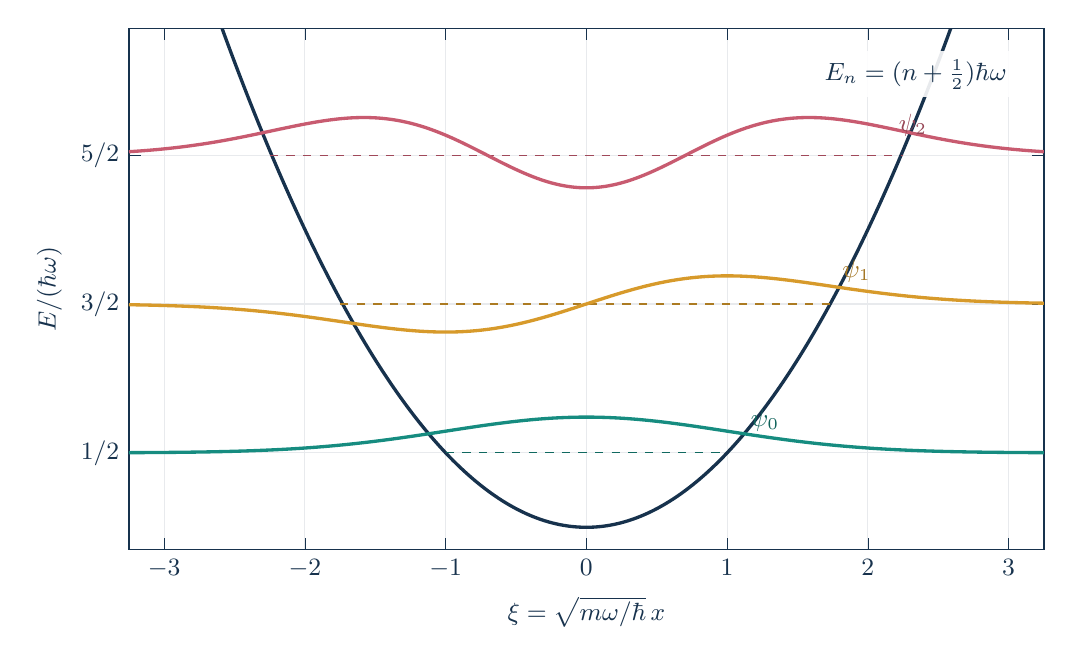
\begin{tikzpicture}
\begin{axis}[
  width=13.2cm,height=8.2cm,
  xmin=-3.25,xmax=3.25,ymin=-0.15,ymax=3.35,
  axis line style={ink,semithick},
  tick style={ink},
  tick label style={font=\small,text=ink},
  label style={font=\small,text=ink},
  xlabel={$\xi=\sqrt{m\omega/\hbar}\,x$},
  ylabel={$E/(\hbar\omega)$},
  xtick={-3,-2,-1,0,1,2,3},
  ytick={0.5,1.5,2.5},
  yticklabels={$1/2$,$3/2$,$5/2$},
  grid=major,grid style={ink!10},
  samples=241,
  domain=-3.25:3.25,
  clip=true
]
  \addplot[very thick,ink] {0.5*x^2};
  \addplot[dashed,teal!75!black] coordinates {(-1,0.5) (1,0.5)};
  \addplot[very thick,teal] {0.5+0.24*exp(-x^2/2)};
  \addplot[dashed,gold!80!black] coordinates {(-1.75,1.5) (1.75,1.5)};
  \addplot[very thick,gold] {1.5+0.22*sqrt(2)*x*exp(-x^2/2)};
  \addplot[dashed,rose!80!black] coordinates {(-2.25,2.5) (2.25,2.5)};
  \addplot[very thick,rose] {2.5+0.11*(4*x^2-2)*exp(-x^2/2)};
  \node[anchor=west,font=\small,text=teal!70!black] at (axis cs:1.1,0.72) {$\psi_0$};
  \node[anchor=west,font=\small,text=gold!75!black] at (axis cs:1.75,1.72) {$\psi_1$};
  \node[anchor=west,font=\small,text=rose!75!black] at (axis cs:2.15,2.7) {$\psi_2$};
  \node[anchor=north east,font=\small,text=ink,fill=white,fill opacity=.9,text opacity=1,inner sep=3pt]
    at (axis cs:3.05,3.2) {$E_n=(n+\tfrac12)\hbar\omega$};
\end{axis}
\end{tikzpicture}
\end{document}
